\section{Clasificación no Supervisada: Análisis Cluster}

\begin{itemize}
    \item Agrupar $n$ individuos en grupos (clusters), tratando de que sean homogeneos en el grupo y con grupos heterogeneos entre si.
    \item Desconocemos la cantidad de grupos que se busca, ni existe una asignación previa en el conjunto de entrenamiento.
    \item \textbf{Métodos Jerárquicos:} Se define una expresión de disimilaridad y se asigna en grupos en función de la distancia, es decir, se ``ordenan'' en función de una/s regla/s (jerarquía).
    \item \textbf{Índice de disimilaridad} $d(x_i,x_{i'})$ mide diferencias entre individuos
    \begin{itemize}
        \item Euclidea: $d_E(x_i,x_{i'})=\|x_i-x_{i'}\|=\sqrt{(x_{i1}-x_{i'1})^2+\cdots+(x_{ip}-x_{i'p})^2}$.
        \item Manhatan o City Block: $d_M(x_i,x_{i'})=|x_{i1}-x_{i'1}|+\cdots|x_{ip}-x_{i'p}|$.
        \item Máximo o Chebyshev: $d_{Ch}(x_i,x_{i'})=\max\{|x_{i1}-x_{i'1}|,\dots,|x_{ip}-x_{i'p}|\}$.
        \item Camberra: Cuando las variables son positivas. $d_C(x_i,x_{i'})=\sum_{j=1}^p\frac{|x_{ij}-x_{i'j}|}{|x_{ij}|+|x_{i'j}|}$.
        \item 1-coseno: Siendo $\alpha$ el ángulo entre los vectores. $d_{\text{1-cos}}(x_i,x_{i'})=1-\cos(\alpha)$.
        
        Si trabajamos con datos ``normalizados'' al centrar por filas ($\tilde{x}_{ij}=x_{ij}-\overline{x}_i)$. $d_{\text{1-cos}}(\tilde{x}_i,\tilde{x}_{i'})=1-\text{Corr}(\tilde{x}_i,\tilde{x}_{i'})$.
        \item Single-matching, Jaccard, Tanimoto, Seath-Sokal: Para variables con niveles binarios.
        \item Distancias para variables categóricas, cadenas (Hamming y Levenshtein), variables mixtas (Gower)\dots
    \end{itemize}
    \item \textbf{Índice de agregación} $\partial(A,B)$ mide diferencias entre grupos
    \begin{itemize}
        \item Single Linkage: $\partial(A,B)=\min_{x\in A,y\in B}d(x,y)$. Afectado por problemas de ``cadena''
        \begin{figure}[h]
            \centering
            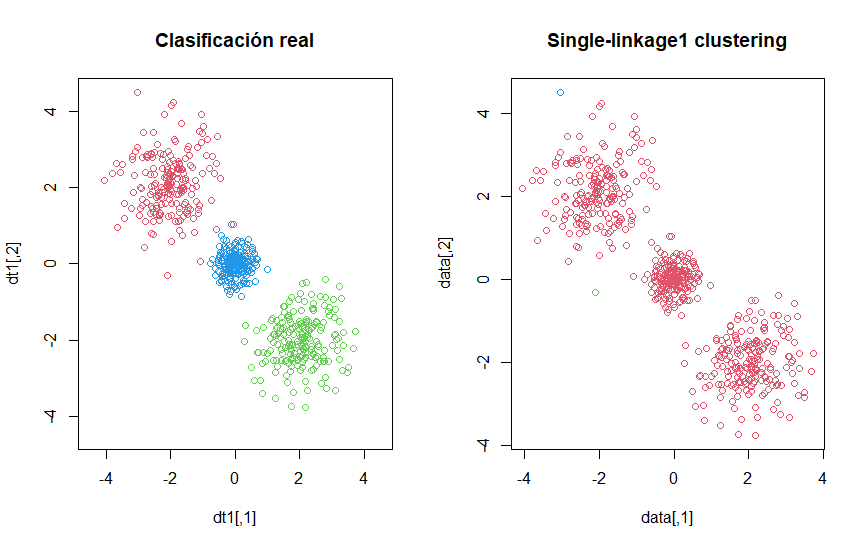
\includegraphics[width=0.8\textwidth]{assets/chain_effect.png}
        \end{figure}
        \newpage
        \item Complete linkage: $\partial(A,B)=\max_{x\in A,y\in B}d(x,y)$.
        \item Método de Ward: El individuo $x$ tiene peso $p(x)$. Si $n_C=\sum_{x\in C}p(x)$ y $g_C=\frac{1}{n_C}\sum_{x\in C}xp(x)$ entonces
        \[
            \partial(A,B)=\frac{n_A n_B}{n_A+n_B}d(g_A, g_B)^2
        \]
    \end{itemize}
    \item \textbf{Dendrograma:} Se unen $A$ y $B$ por etapas donde en cada etapa, $\partial(A,B)$ sea la más pequeña. Se repite el proceso hasta que no queden observaciones. Para crear los grupos se ``corta'' el árbol.
    \begin{figure}[h]
        \centering
        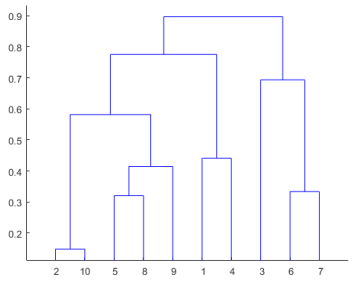
\includegraphics[width=0.5\textwidth]{assets/dendograma.png}
    \end{figure}
    \item \textbf{Métodos no Jerárquicos:} Se fija el número de grupos a buscar y se optimiza algún criterio, como por ejemplo la media de los grupos.
    \item \textbf{Método de $k$-medias:} Se buscan $k$ centros óptimos $m_1^*,\dots,m_k^*$ en $\mathbb{R}^p$.
    \item Algoritmo: Se seleccionan $k$ centros al azar $c_1^0,\dots,c_k^0$ y se crean particiones $I_1^0,\dots,I_k^0$ por cercanía. Despues se calcula la media de cada partición y se asignan como nuevos centros $c_1^1,\dots,c_k^1$. Se repite el proceso hasta estabilizarse ($I_j^{k-1}=I_j^k$).
    \begin{figure}[h]
        \centering
        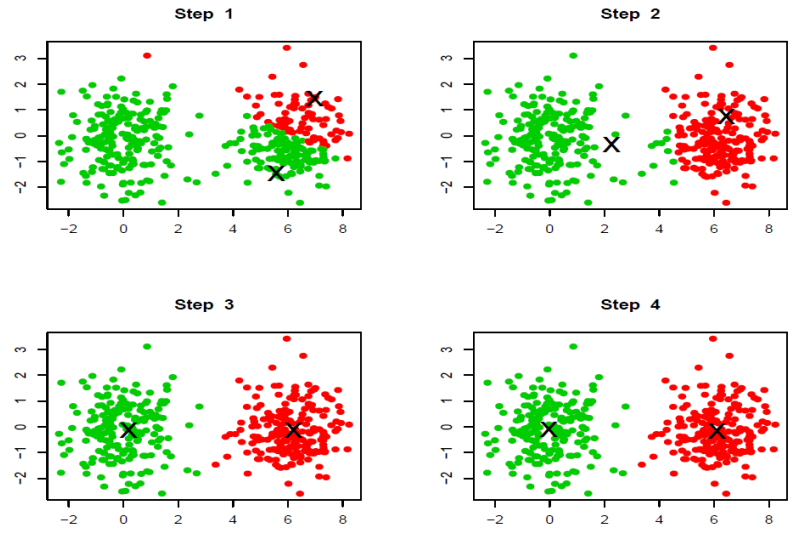
\includegraphics[width=0.8\textwidth]{assets/k_means.png}
    \end{figure}
    \newpage
    \item Las $k$-medias tienen preferencia por clusters esféricos y con dispersiones parecidas.
    \item \textbf{Métodos basados en modelos:} Métodos más flexibles, como la maximización de la verosimilitud de ``clasificación'' o la maximización de la verosimilitud tipo ``mixtura''.
    \item Las $k$-medias son un tipo especial de la maximización de la verosimilitud de ``clasificación''.
    \item Lo del final no se si ponerlo xd.
    \item Mapa de calor: Matriz de distancias. Representa en cada elemento $ij$ la distancia entre el individuo $i$ y el $j$ (lo pongo al final por que se me olvidó antes y asi relleno la página ole).
    \begin{figure}[h]
        \centering
        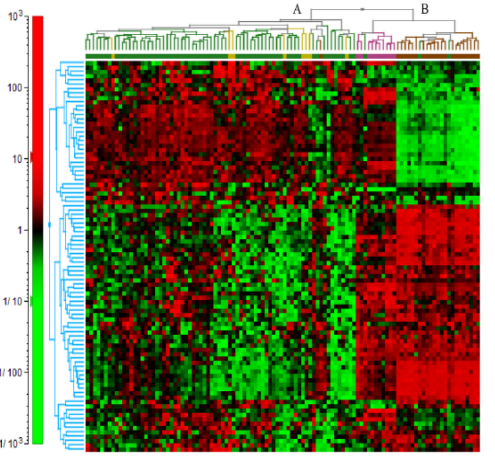
\includegraphics[width=\textwidth]{assets/mapa_calor.png}
    \end{figure}
\end{itemize}